\begin{frame}{2. L'apprentissage supervisé}
  \begin{itemize}
  \item Utilise des données \textit{labélisées}
  \item La machine apprend par l'exemple
  \item \textit{Prédis} le résultat pour de nouveaux événements
  \item Problèmes de régression et de classification
  \item Regression linéaire et logistique
  \item Réseaux de Neurones
  \item Arbres de décisions
  \end{itemize}
\end{frame}

\begin{frame}{2.1 La régression linéaire}
  \begin{itemize}
  \item Mais... À quoi ça sert en vrai?
    \begin{itemize}
    \item Prédiction d'une valeur en fonction de paramètres (prix de quelque chose)
    \item Très utilisé en science (physiques des particules, sciences sociales) pour mettre en évidence des relations entre des variables ou ajuster un modèle
    \item Dans le domaine médicales: les études épidémiologique
    \item Dans la finance: prédictions des tendances, \textit{Capital Asset Pricing Model}
    \item $\dots$
    \end{itemize}
  \end{itemize}
\end{frame}

\begin{frame}{2.1 Un exemple: le prix d'une carte graphique}
  \begin{itemize}
  \item Ce prix va dépendre de la taille de la mémoire vive (GPU) de la carte (entre autre ...)
    \vspace{0.2cm}
  \item On a un jeu de données, cad une liste de carte graphique dont on connait le couple $\{GPU;prix\}$:
  \end{itemize}

  \begin{figure}
    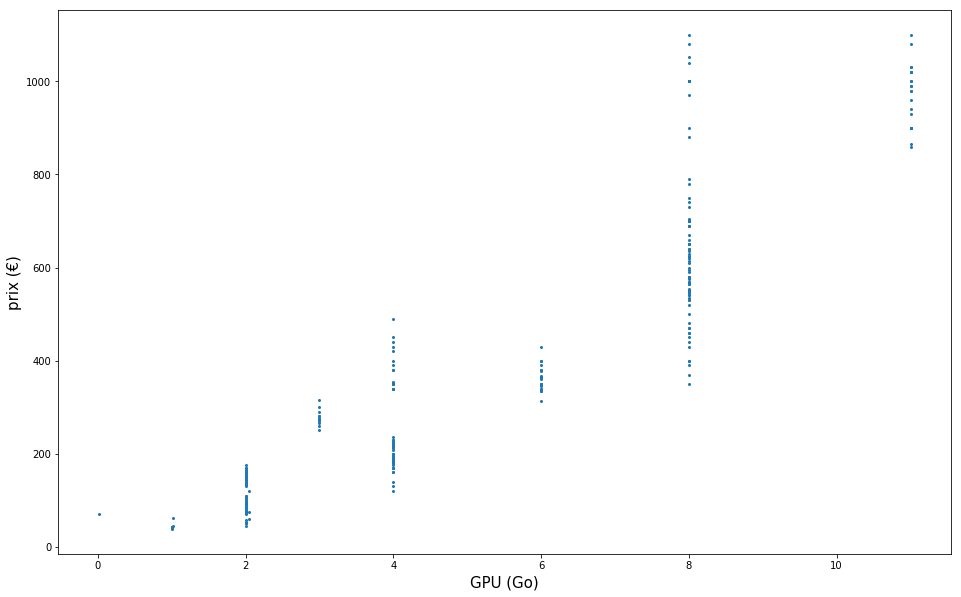
\includegraphics[width=0.8\textwidth]{fig/gpuPrices.png}    
  \end{figure}
\end{frame}

\begin{frame}{2.1 Construire un modèle (regression linéaire)}
  \begin{itemize}
  \item Appelons $x_{1}$ la taille de la mémoire vive de nos $m$ carte graphiques, et $y$ le prix correspondant.
    \vspace{0.2cm}
  \item On cherche à trouver le modèle qui permet de prédire un prix $\hat{y}$ à partir $x_{1}$:
    \begin{equation*}
      \hat{y} = h_{\theta}(x_{1})
    \end{equation*}
  \item On défini le paramètre $\theta_{1}$ qui va \textit{lier} $x_{1}$ à $\hat{y}$:
    \begin{equation*}
      h_{\theta}(x) = \theta_{1} x_{1}
    \end{equation*}
  \item Rappel math: \textbf{fonction linéaire} $f(x) = kx$
  \end{itemize}
\end{frame}

\begin{frame}{2.1 Construire un modèle (regression linéaire)}
  \begin{itemize}
  \item Initialisons aléatoirement la valeur de $\theta_{1}$
  \end{itemize}
  \vspace{-0.5cm}
  \begin{figure}
    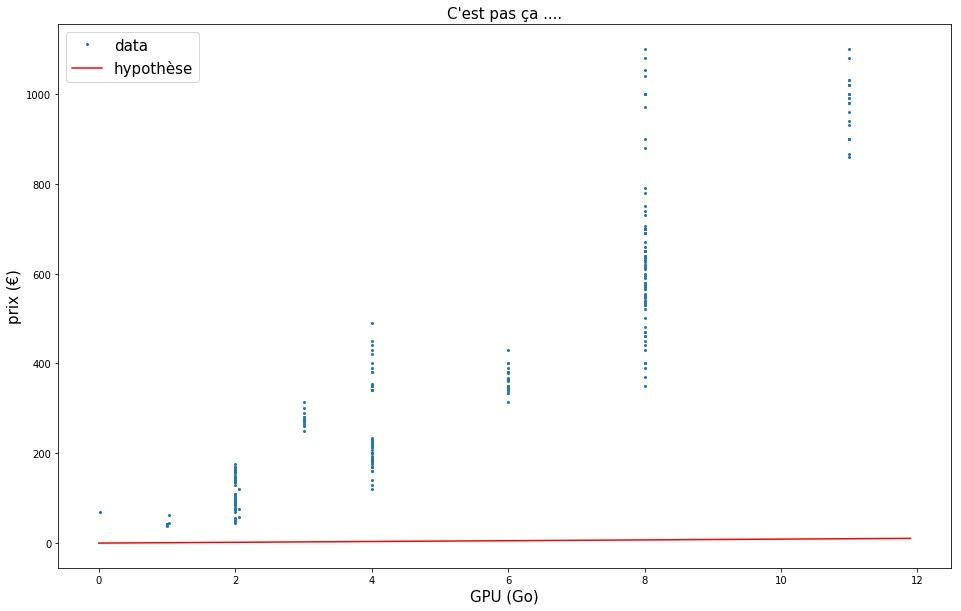
\includegraphics[width=0.8\textwidth]{fig/model.png}
  \end{figure}
  \vspace{-0.5cm}
  \begin{itemize}
  \item C'est pas encore ça ...
  \end{itemize}
\end{frame}

\begin{frame}{2.1 La fonction de coût}
  \begin{itemize}
  \item Comment estimer la \textit{véracité} de notre modèle?
    \begin{itemize}
    \item La \textbf{Fonction de coût}: $J(\theta)$
      \vspace{0.15cm}
    \item Une définition possible: somme quadratique des erreurs
      \begin{equation*}
        J(\theta) = \frac{1}{2m} \displaystyle\sum_{i=0}^{m}(\hat{y}^{(i)} - y^{(i)})^{2}
      \end{equation*}
    \end{itemize}
  \end{itemize}
  \vspace{-0.5cm}
  \begin{figure}
    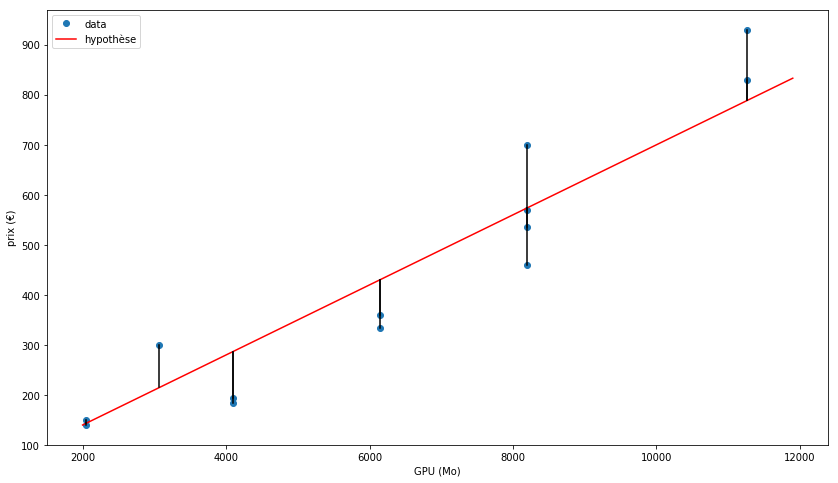
\includegraphics[width=0.8\textwidth]{fig/modelEstimation.png}
  \end{figure}  
\end{frame}

\begin{frame}{2.1 La fonction de coût}
  \begin{itemize}
  \item On cherche à trouver la valeur de $\theta_{1}$ qui \textbf{minimise} $J(\theta)$
    \vspace{0.2cm}
  \item En Brute ...
  \end{itemize}
  \vspace{-0.5cm}
  \begin{figure}
    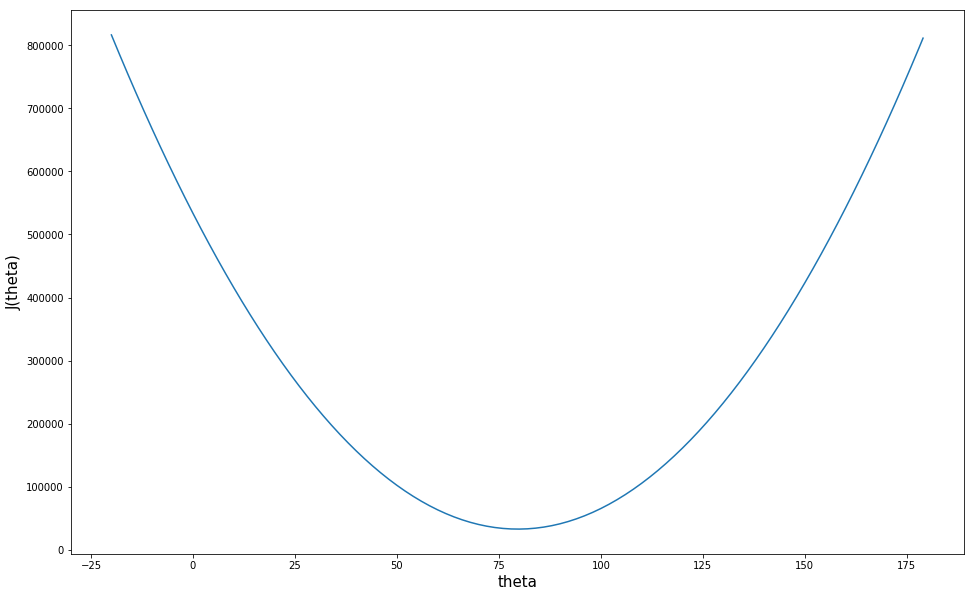
\includegraphics[width=0.8\textwidth]{fig/costFct.png}
  \end{figure}
  \vspace{-0.5cm}
  \begin{itemize}
  \item ... essayons d'optimiser
  \end{itemize}
\end{frame}

\begin{frame}{2.1 La descente de gradient}
  \begin{itemize}
  \item C'est l'algorithme qui va nous permettre d'arriver ``\textit{rapidement}'' au minimum de $J(\theta)$ 
    \vspace{0.2cm}
  \item On va utiliser la \textit{dérivation}: $\frac{d}{d\theta_{1}}J(\theta)$:
    \begin{itemize}
    \item Si $J(\theta)$ est croissant: $\frac{d}{d\theta_{1}}J(\theta) > 0$
    \item Si $J(\theta)$ est décroissant: $\frac{d}{d\theta_{1}}J(\theta) < 0$
    \end{itemize}
  \end{itemize}
  \vspace{-0.5cm}
  \begin{figure}
    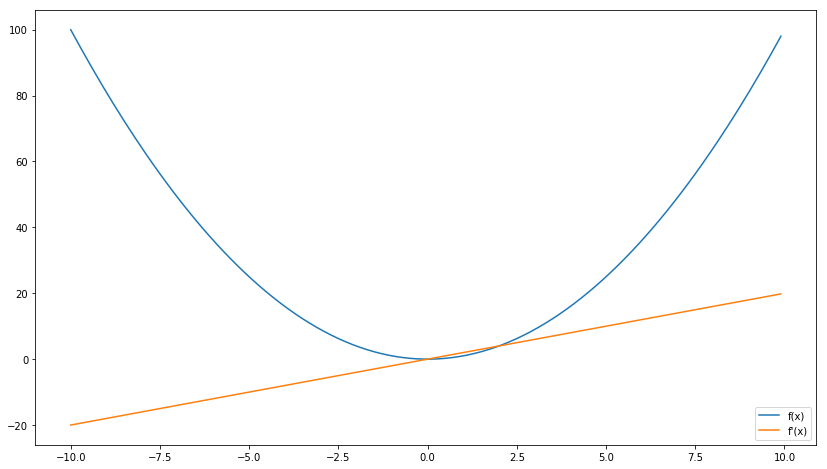
\includegraphics[width=0.7\textwidth]{fig/derivation.png}
  \end{figure}
  \vspace{-0.5cm}
\end{frame}


\begin{frame}{2.1 La descente de gradient}
  \begin{itemize}
  \item (Encore) un peu de math, la descente de gradient s'écrit:
  \end{itemize}
  \begin{beamerboxesrounded}[scheme=suppervise,width=\textwidth]{\textcolor{black}{Descente de gradient}}    
    \vspace{-0.2cm}
    \begin{equation*}
      \begin{matrix} \text{Répéter jusqu'à convergence:} & \{ & \\ & & \theta_{1} := \theta_{1} - \alpha \frac{d}{d\theta_{1}}J(\theta) \\ & \} & \end{matrix}
    \end{equation*}
    \vspace{-0.2cm}
  \end{beamerboxesrounded}
  \begin{itemize}
  \item $\alpha$ s'appelle le taux d'apprentissage (\textit{learning rate}) et c'est le \textbf{seul} paramètre de l'algorithme.
    \vspace{0.2cm}
  \item On va itérativement modifier la valeur de $\theta_{1}$ en fonction de la dérivée de $J(\theta)$, jusqu'à minimiser $J(\theta)$ (\textit{convergence}).
  \end{itemize}
\end{frame}

\begin{frame}{2.1 La descente de gradient}
  \begin{itemize}
  \item Dérivons donc notre fonction de coût:
  \end{itemize}
  \begin{equation*}
    J(\theta) = \frac{1}{2m} \displaystyle\sum_{i=0}^{m}(\hat{y}^{(i)} - y^{(i)})^{2} = \frac{1}{2m} \displaystyle\sum_{i=0}^{m}(\theta_{1}x_{1}^{(i)} - y^{(i)})^{2}
  \end{equation*}
  \begin{equation*}
    \frac{d}{d\theta_{1}}J(\theta) = \frac{1}{m}\displaystyle\sum_{i=0}^{m}(\hat{y}^{(i)} - y^{(i)}) x_{1}^{(i)}
  \end{equation*}
  \begin{itemize}
  \item Un peu de \textit{hand-tunning}:
    \begin{itemize}
    \item Le learning rate ($\alpha$) est fixé à $0.00000003$
    \item Défissons une précision $\epsilon = 0.001$ qui nous servira a arrêter la descente de gradient 
    \end{itemize}
  \end{itemize}
\end{frame}

\begin{frame}{2.1 C'est parti !}
  \begin{figure}
    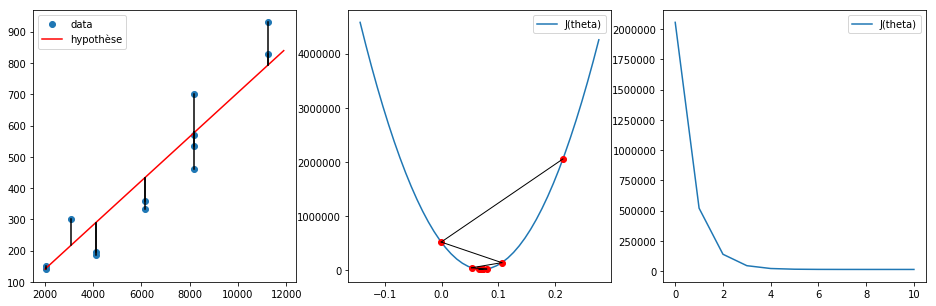
\includegraphics[width=\textwidth]{fig/gradDescent.png}
  \end{figure}
  \begin{itemize}
  \item La descente de gradient c'est achevée au bout d'une dizaine d'itérations
  \item La valeur de notre paramètre $\theta_{1}$ est $0.0706$
  \item On peut voir que $J(\theta)$ a continuellement diminué à chaque itération
  \end{itemize}
\end{frame}

\begin{frame}{2.1 On peut maintenant faire une prédiction}
  \begin{itemize}
  \item Quel serait le prix d'une carte avec 4608 et 13516 Mo de GPU? (ce qui n'a pas de sens, on est d'accord)
  \end{itemize}
  \vspace{-0.2cm}
  \begin{figure}
    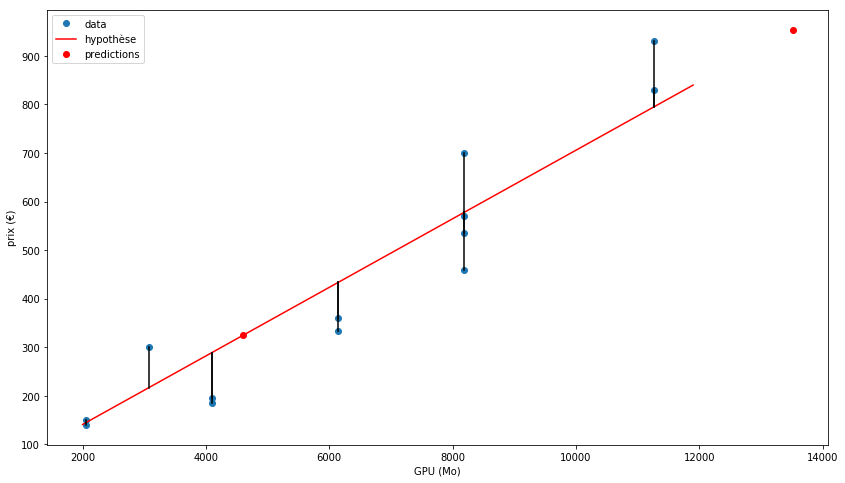
\includegraphics[width=0.8\textwidth]{fig/pred.png}
  \end{figure}
  \vspace{-0.5cm}
  \begin{itemize}
  \item On pourra les vendre autour de 325.10 et 953.62 euros !
  \end{itemize}
\end{frame}

\begin{frame}{2.1 Le choix du taux d'apprentissage}
  \begin{itemize}
  \item \textbf{\textcolor{orange}{Learning Rate} Très important:}
    \begin{itemize}
      \normalsize
    \item \boldmath $\alpha$ \textbf{Trop grand:} la descente de gradient diverge
    \item \boldmath $\alpha$ \textbf{Trop petit:} la descente de gradient est très longue
    \end{itemize}
  \item Pour choisir, on regarde l'évolution de la fonction de coût $J(\theta)$ en fonction du nombre d'itérations:
  \end{itemize}
  \vspace{-0.5cm}
  \begin{figure}
    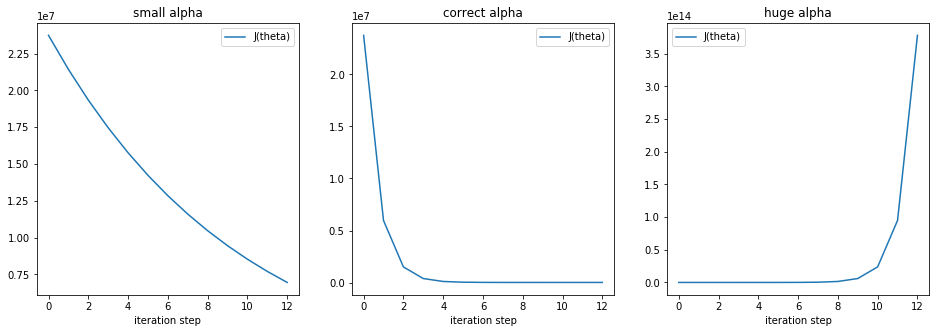
\includegraphics[width=0.9\textwidth]{fig/learningRateChoice.png}
  \end{figure}
\end{frame}

\begin{frame}{2.1 Un mot sur la regression linéaire multivariables}
  \begin{itemize}
  \item Ici, nous avons vu le cas avec une seule variable $x_{1}$ (on aurait pu rajouter un biais $\theta_{0}$, cad un terme constant: $\hat{y} = \theta_{0} + \theta_{1}x_{1}$)
  \item Le principe est le même, mais avec plusieurs variables $x_{i}$ (donc plusieurs paramètres $\theta_{i}$)
  \item Notre fonction hypothèse s'écrie alors:
  \end{itemize}
  \begin{equation*}
    h_{\theta}(x) = \theta_{0} + \theta_{1}x_{1} + \theta_{2}x_{2} + \dots + \theta_{n}x_{n} = \theta_{0} + \displaystyle\sum_{i=1}^{n} \theta_{i} x_{i}
  \end{equation*}
  \begin{itemize}
    \item \textbf{\textcolor{orange}{Astuce:}} On définit $x_{0} = 1$, et on re-écrit la fonction hypothèse:
  \end{itemize}
  \begin{equation*}
    h_{\theta}(x) = \theta_{0}x_{0} + \theta_{1}x_{1} \dots + \theta_{n}x_{n} = \displaystyle\sum_{i=0}^{n} \theta_{i} x_{i}
  \end{equation*}

  \begin{itemize}
  \item La fonction de coût reste inchangée
  \end{itemize}
\end{frame}

\begin{frame}{2.1 Un mot sur la regression linéaire multivariables}
  \begin{itemize}
  \item Dans le cas multivariables, la descente de gradient devient:
  \end{itemize}
    \begin{beamerboxesrounded}[scheme=suppervise,width=\textwidth]{\textcolor{black}{Descente de gradient (cas multivariables)}}    
    \vspace{-0.2cm}
    \begin{equation*}
      \begin{matrix} \text{Répéter jusqu'à convergence:} & \{ & \\
        & & \theta_{0} := \theta_{0} - \alpha \frac{d}{d\theta_{0}}J(\theta) \\
        & & \theta_{1} := \theta_{1} - \alpha \frac{d}{d\theta_{1}}J(\theta) \\
        & & \theta_{2} := \theta_{2} - \alpha \frac{d}{d\theta_{2}}J(\theta) \\
        & & \dots \\
        & \} & \end{matrix}
    \end{equation*}
    \vspace{-0.2cm}
  \end{beamerboxesrounded}
    \begin{itemize}
    \item Il est très important de simultanément changer les valeurs des paramètres.
    \end{itemize}
\end{frame}

\begin{frame}{2.1 Un mot sur la regression linéaire multivariables}
  \begin{itemize}
  \item Pour illustrer: régression linéaire à deux dimensions
  \end{itemize}
  \begin{figure}
    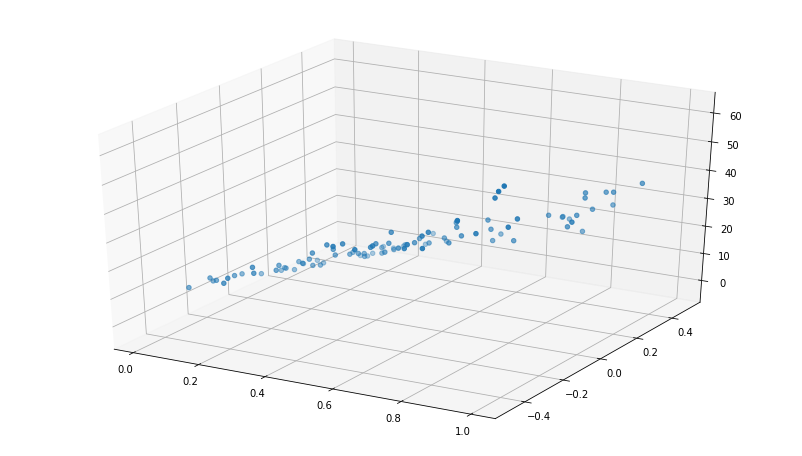
\includegraphics[width=0.45\textwidth]{fig/multiVarData.png}
    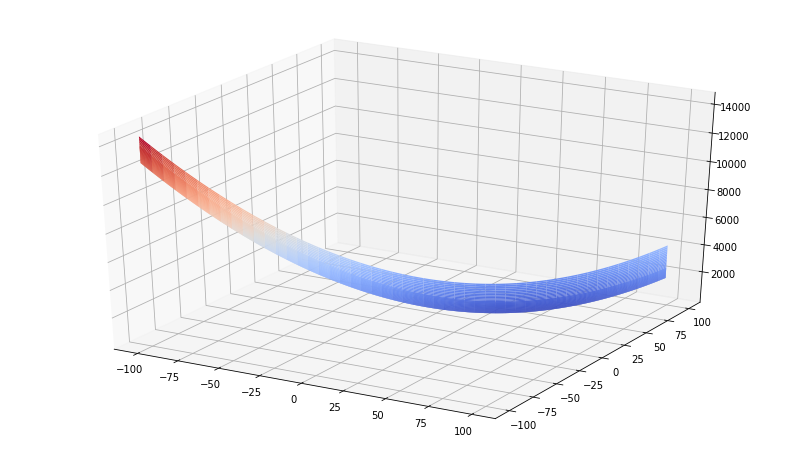
\includegraphics[width=0.45\textwidth]{fig/multiVarCostFct.png}\\
    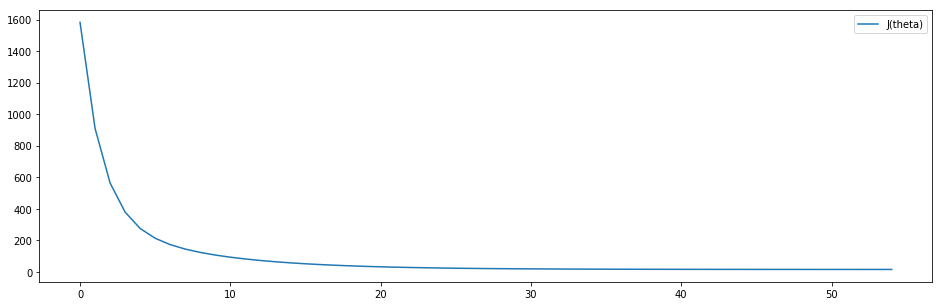
\includegraphics[width=0.75\textwidth]{fig/multiVarDesc.png}
  \end{figure}
\end{frame}

\begin{frame}{2.1 Features scaling}
  \begin{itemize}
  \item Lorsque les variables n'ont pas la même échelle, la descente de gradient peut prendre beaucoup de temps
  \item Normaliser les variables: $-1 \leq x_{i} \leq 1$
  \end{itemize}
  \vspace{-0.2cm}
  \begin{table}
    \footnotesize
        {\def\arraystretch{2}\tabcolsep=8pt
          \begin{tabular}{l|l|l}
            & \textbf{Feature Scaling} & \textbf{Mean normalization}\\
            \hline
            \textbf{Start range} & $x_{min} \leq x \leq x_{max}$ & $x_{min} \leq x \leq x_{max}$ \\
            \textbf{Transformation} & $x := \frac{x - x_{min}}{x_{max} - x_{min}}$ & $x := x - x_{mean}$ \\
            \textbf{New range} & $0 \leq x \leq 1$ & $(x_{min}-x_{mean}) \leq x \leq (x_{max}-x_{mean})$
          \end{tabular}
        }
  \end{table}
  \vspace{-0.2cm}
  \begin{itemize}
  \item En combinant les deux: \boldmath \textcolor{orange}{$x := \frac{x - x_{mean}}{x_{max} - x_{min}}$} $\Rightarrow$ \textcolor{orange}{$-1 \leq x \leq 1$} 
    \vspace{0.2cm}
    \footnotesize
  \item\textbf{Remarque:} Il est possible de remplacer $x_{max} - x_{min}$ par l'écart type:
  \end{itemize}
  \footnotesize
  \begin{equation*}
    \sigma_{x} = \sqrt{\frac{1}{n}\displaystyle\sum_{i=1}^{n}(x_{i} - \bar{x})^{2}}
  \end{equation*}
\end{frame}

\begin{frame}{2.2 La régression logistique}
  \begin{itemize}
  \item \textbf{\textcolor{orange}{Classification}}: prédire un nombre limités de valeurs discrètes
    \begin{itemize}
    \item \textbf{Classification binaire}: Deux valeurs possibles: Vrai ou Faux (spam / non spam)
    \item \textbf{Classification multiclasse}: plusieurs valeurs possibles (camion, voiture, piétons, vélos, ...)
    \end{itemize}
    \vspace{0.5cm}
  \item \textcolor{orange}{\textbf{Classification binaire:}} En utilisant la régression linaire?
    \begin{itemize}
    \item $y \in \{0,1\}$ \textcolor{orange}{$\Rightarrow$} On défini un seuil $S$ pour $h_{\theta}(x)$:
      \begin{equation*}
        \begin{matrix*}[l]
          h_{\theta}(x) \geq S \rightarrow y = 1\\
          h_{\theta}(x) < S \rightarrow y = 0
        \end{matrix*}
      \end{equation*}
    \end{itemize}
  \item \textbf{Problème:} On voudrait que $0 \leq h_{\theta}(x) \leq 1$
  \end{itemize}
  \begin{center}
    $\Rightarrow$ Il faut redéfinir notre fonction hypothèse!
  \end{center}
\end{frame}

\begin{frame}{2.2 La régression logistique}
  \begin{itemize}
  \item Modèle de la régression logistique:
    \begin{itemize}
      \item On utilise la \textbf{Fonction Sigmoïde} $g(z)=\frac{1}{1+e^{-z}}$
    \end{itemize}
  \end{itemize}
  \begin{minipage}{0.4\textwidth}
    \begin{equation*}
      \begin{matrix*}[l]
        z = \displaystyle\sum_{i=0}^{n} \theta_{i} x_{i}\\
        h_\theta(x) = g(z) \\
      \end{matrix*}
    \end{equation*}
    \vfill
    \begin{equation*}
      \textcolor{blue}{0 \leq h_{\theta}(x) \leq 1}
    \end{equation*}
  \end{minipage}
  \begin{minipage}{0.5\textwidth}
    \begin{figure}
      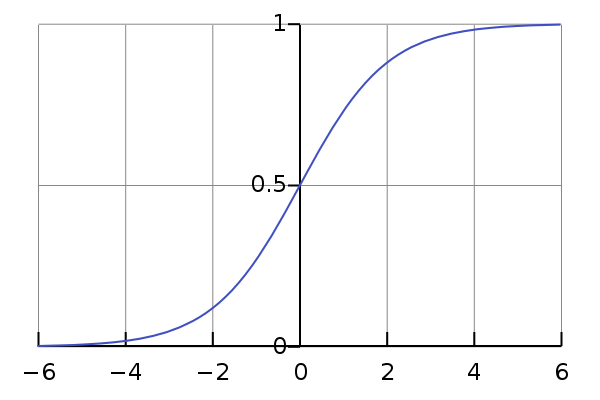
\includegraphics[width=0.9\textwidth]{fig/logisticFct.png}
    \end{figure}
    \begin{center}
      \tiny
      \vspace{-0.5cm}
      \textcolor{blue}{$g(z)$} depuis \href{https://en.wikipedia.org/wiki/Sigmoid_function}{\color{blue}{Wikipedia}}
    \end{center}
  \end{minipage}
  \vfill
  \begin{itemize}
  \item \textbf{Classification:} On prédit une \textbf{probabilité}
  \end{itemize}
\end{frame}

\begin{frame}{2.2 La régression logistique}
  \begin{itemize}
  \item On change également la fonction de coût:
  \end{itemize}
  \begin{equation*}
    J(\theta)=\frac{1}{m} \displaystyle \sum_{i=1}^{m}Cost(h_{\theta}(x^{(i)}),y^{(i)})
  \end{equation*}
  \begin{itemize}
  \item Avec:
  \end{itemize}
  \begin{equation*}
    Cost(h_{\theta}(x),y) = 
    \begin{cases}
      -log(h_{\theta}(x)) & \quad \text{if } y = 1 \\
      -log(1 - h_{\theta}(x)) & \quad \text{if } y = 0 \\
    \end{cases}
  \end{equation*}
  \begin{figure}
    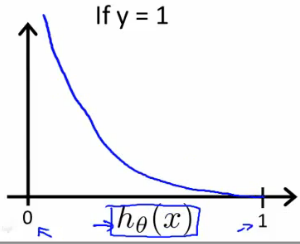
\includegraphics[width=.35\textwidth]{fig/logisticRegressionCostFunction1.png}
    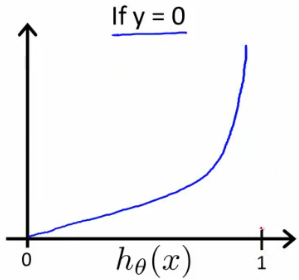
\includegraphics[width=.32\textwidth]{fig/logisticRegressionCostFunction2.png}
  \end{figure}
\end{frame}

\begin{frame}{2.2 La régression logistique}
  \begin{itemize}
  \item Et la \textcolor{orange}{\textbf{Classification multiclasse}} ? $y \in \{0,1,2,\dots,n\}$
  \item La \textbf{descente de gradient} ne permet pas de la résoudre
  \item On peut \textit{tricher} en utilisant la méthode \textit{'One-vs-all'}:
    \begin{itemize}
    \item On remplace le problème multiclasse par $n+1$ problèmes binaire
    \item Probabilité que $y$ soit dans une classe, les autres sont regroupés dans une deuxième classe \textit{virtuelle}:
    \end{itemize}
  \end{itemize}
  \begin{equation*}
    \begin{matrix*}[l]
      h_{\theta}^{(0)} = P(y=0 | x;0)\\
      h_{\theta}^{(1)} = P(y=1 | x;0)\\
      \dots \\
      h_{\theta}^{(n)} = P(y=n | x;0)\\
      \text{prediction} = max_{i}(h_{\theta}^{(i)}(x))\\
    \end{matrix*}
  \end{equation*}
  \begin{itemize}
  \item Algorithme d'optimisation avancés: \textit{Conjugate gradient}, \textit{(L-)BFGS}, $\dots$
  \end{itemize}
\end{frame}

\begin{frame}{2.3 Les problèmes de biais et de variance}
  \begin{figure}
    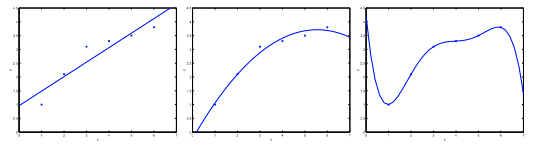
\includegraphics[width=0.9\textwidth]{fig/theProblemOfOverfitting.png}
  \end{figure}
  \footnotesize
  \vspace{-1cm}
  \begin{center}
    \textit{Underfitting} (Bias) \hspace{1.5cm} \textit{Just fine!} \hspace{1.5cm} \textit{Overfitting} (Variance)
  \end{center}
  \begin{itemize}
  \item \textbf{Underfitting}: modèle trop simple (pas assez de variables)
  \item \textbf{Overfitting}: modèle trop complexe, deux manière de résoudre:
    \begin{itemize}
    \item Réduire le nombres de variables ou changer les paramètres du modèle
    \item Utiliser des méthodes de \textbf{régularisation}
    \end{itemize}
  \end{itemize}  
\end{frame}

\begin{frame}{2.3 La régularisation}
  \begin{itemize}
  \item Contraindre les paramètres $\theta_{j}$ sans réduire le nombre de variables
  \item On ré-écrit la fonction de coût avec le \textcolor{blue}{terme de régularisation}:
  \end{itemize}
  \begin{equation*}
    J(\theta) = \frac{1}{2m}(\displaystyle\sum_{i=1}^{m}(h_{\theta}(x^{(i)}) - y^{(i)})^{2} + \textcolor{blue}{\lambda \displaystyle\sum_{j=1}^{n}\theta_{j}^{2}})
  \end{equation*}
  \begin{itemize}
  \item \boldmath $\lambda$: Paramètre de régularisation
  \item Si $\lambda$ est trop grand: risque d'\textit{underfitting}
  \item Si $\lambda = 0$: pas de régularisation. 
  \item \textbf{Remarque:} On ne régularise pas le terme constant $\theta_{0}$
  \end{itemize}
\end{frame}

\begin{frame}{2.4 Les arbres de décisions}
  \begin{itemize}
  \item Effectue une prédiction (regression ou classification) par une succession de decision simples: \textit{if-else-then} sur les différentes variables
  \item \textit{Arbre} = suite de décisions (\textit{noeuds}) ammenant à une prédiction (\textit{feuille})
  \end{itemize}
  \begin{minipage}{.45\textwidth}
    \begin{itemize}
    \item La complexité de la structure de données qu'il est possible de représenter avec une arbre de décision est proportionelle à la profondeur de l'arbre
    \end{itemize}
  \end{minipage}
  \begin{minipage}{.54\textwidth}
    \begin{figure}
      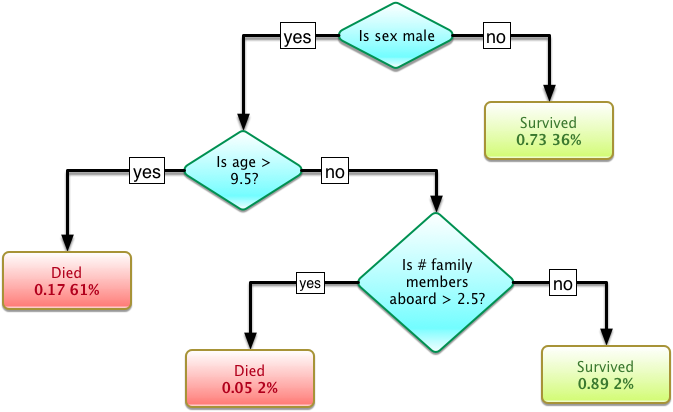
\includegraphics[width=.9\textwidth]{fig/decisionTreeExample.png}
    \end{figure}
    \begin{center}
      \scriptsize
      \textit{Un arbre pour déterminer la probabilité de survie des passagers du Titanic (depuis \href{https://en.wikipedia.org/wiki/Decision_tree_learning}{\color{blue}{Wikipedia}})}
    \end{center}
  \end{minipage}
\end{frame}

\begin{frame}{2.4 Les arbres de décisions: Apprentissage}
  \begin{itemize}
  \item La \textit{meilleure} séparation possible est déterminée:
    \begin{itemize}
      \normalsize
    \item Toutes les variables/sélection possibles
    \item Celle qui minimise une fonction de coût
    \end{itemize}
  \item L'échantillon d'entrainement est séparé suivant cette décision, créant ainsi deux feuilles (sous-échantillon)
  \item On recommence l'opération tant que l'on a pas atteint la profondeur voulue ou bien que la pureté de chaque feuille atteint un niveau satisfaisant (à déterminer)
  \end{itemize}
  \vspace{1cm}
  \textbf{Remarque:} Il est possible d'utiliser la même variables pour différents noeud.
\end{frame}

\begin{frame}{2.4 Les arbres de décisions}
  \begin{itemize}
  \item Ces algorithmes sont faciles à interpréter (et à visualiser)
  \item Tout les types de données (catégorielle, numérique, ...) peuvent être mélangés
  \item Rapide et peu gourmand en ressource pour comprendre des structures de données complexes:
  \end{itemize}
  \begin{figure}
    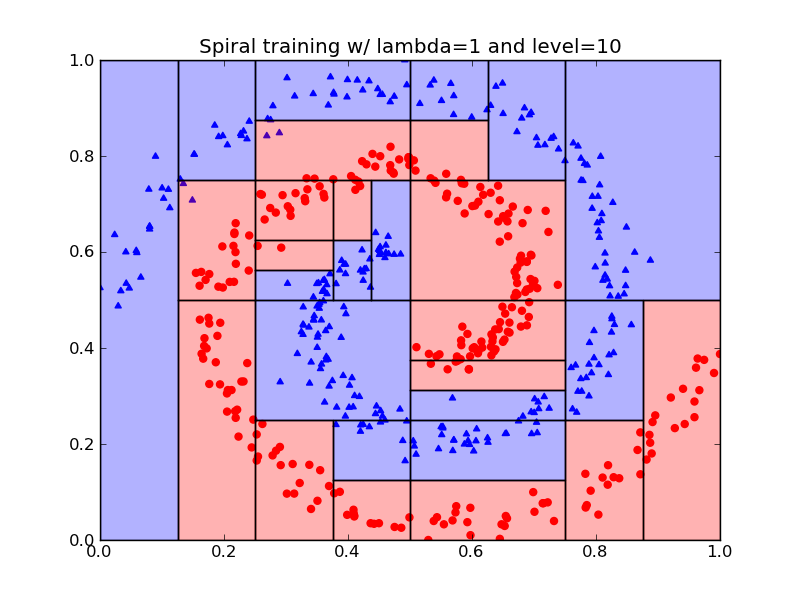
\includegraphics[trim={0 0 0 40},clip,width=.3\textwidth]{fig/spiralDTresult.png}
    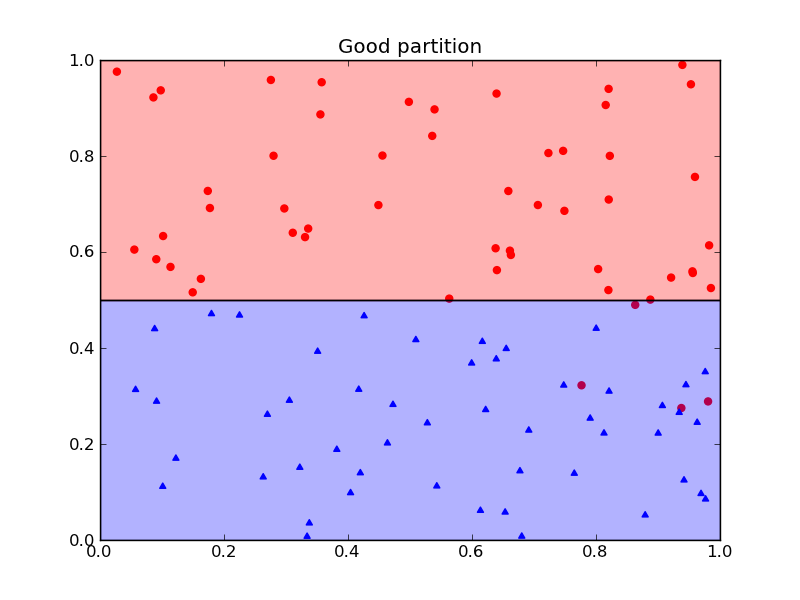
\includegraphics[trim={0 0 0 40},clip,width=.3\textwidth]{fig/goodPartitionDT.png}
    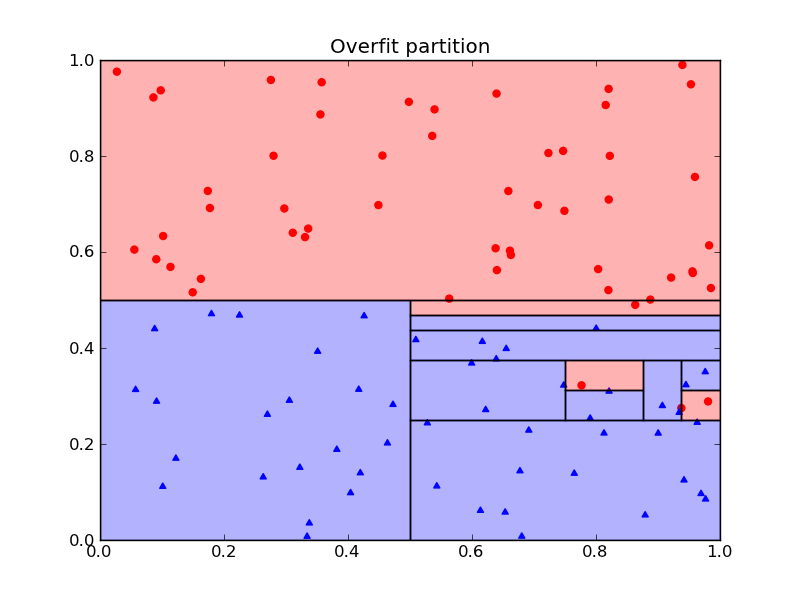
\includegraphics[trim={0 0 0 40},clip,width=.3\textwidth]{fig/overfittingPartitionDT.png}
  \end{figure}
  \vspace{-1cm}
  \begin{center}
    \scriptsize
    \textit{Illustration depuis \href{https://www.classes.cs.uchicago.edu/archive/2013/winter/12200-1/assignments/pa4/index.html}{\color{blue}{University of Chicago}}}
  \end{center}
  \begin{itemize}
  \item Risque d'\textit{overfitting} (sur-apprentissage) du modèle qui se généralise mal
  \item Algorithmes très sensibles au jeu de données d'entrainement
  \end{itemize}
\end{frame}

\begin{frame}{2.4 Les arbres de décisions: méthodes d'ensemble}
  \begin{itemize}
  \item Pour pallier les faiblesse des arbres de décision, on les utilise comme \textit{base learners} dans des méthodes qui en regroupe plusieurs
  \item Il existe deux familles de méthodes:
    \begin{itemize}
      \normalsize
      \vspace{0.5cm}
    \item \textbf{averaging}: plusieurs estimateurs (\textit{learners}) indépendant dont on moyenne les prédictions \\ (\textit{Random Forests}, $\dots$)
      \vspace{0.5cm}
    \item \textbf{boosting}: plusieurs estimateurs combinés \\(\textit{AdaBoost}, \textit{XGBoost}, $\dots$)
    \end{itemize}
  \end{itemize}
\end{frame}

\begin{frame}{2.4 Exemple d'algorithme d'\textit{averaging}: \textbf{Random Forests}}
  \begin{itemize}
  \item \textit{Bagging}: Chaque estimateur (arbre) de l'ensemble est construit à partir d'un sous-échantillon aléatoire (avec replacement) de l'échantillon d'entrainement (\textit{Bootstrap aggregating})
  \item \textit{Features bagging}: La \textit{meilleure} séparation possible sur un sous-échantillon aléatoire des variables
  \item Soit $f_{b}$, l'arbre entrainé sur le sous-échantillons $b$ ($b \in[1,B]$), on calcule la prédiction globale en moyennant les prédictions de tout les arbres:
  \end{itemize}
  \begin{equation*}
    \hat{f} = \frac{1}{B}\displaystyle\sum_{b=1}^{B} f_{b}(x)
  \end{equation*}
  \begin{itemize}
  \item Cette méthode obtient de meilleure performance car elle réduit la \textit{variance} du modèle sans accroitre le \textit{biais}
  \end{itemize}
\end{frame}

\begin{frame}{2.4 Exemple d'algorithme de \textit{boosting}: \textbf{AdaBoost}}
  \begin{itemize}
  \item L'apprentissage d'un même \textit{learner} est répété en modifiant le jeu de données à chaque itération
  \item On utilise des poids: $w_{i}$ pour $i \in [1,N]$. Initialement: $w_{i} = 1/N$
  \item À chaque itération, le poids des exemples correctement prédits diminue tandis que celui des exemples dont les prédictions sont fausse augmente
  \item L'algorithme devient plus sensibles aux exemples difficiles à prédire
  \end{itemize}
\end{frame}

\begin{frame}{2.4 Exemple d'algorithme de \textit{boosting}: \textbf{XGBoost}}
  \begin{itemize}
  \item Obtient d'excellent résultats sur la plupart des cas d'usages (classification et régression)
  \item Des arbres sont générés aléatoirement comme pour les \textit{random forests}
  \item Mais au lieu de moyenner les prédictions, on additionne les prédictions
    \begin{itemize}
    \item À chaque étape, des arbres sont générés et on sélectionne celui qui optimise la fonction d'objectif (une fonction de coût + une fonction qui mesure la complexité du modèle)
    \item On additionne la prédiction de cet arbre à la prédiction du modèle et on recommence jusqu'à atteindre une performance suffisante
    \end{itemize}
  \end{itemize}
  \begin{equation*}
    \begin{matrix*}[l]
      \hat{y_{i}}^{(0)} = 0 \\
      \hat{y_{i}}^{(1)} = \hat{y_{i}}^{(0)} + f_{1}(x_{i}) = f_{1}(x_{i})\\
      \hat{y_{i}}^{(2)} = \hat{y_{i}}^{(1)} + f_{2}(x_{i}) = f_{1}(x_{i}) + f_{2}(x_{i})\\
      \dots\\
      \hat{y_{i}}^{(t)} = \hat{y_{i}}^{(t-1)} + f_{t}(x_{i}) = \displaystyle\sum_{k=1}^{t} f_{k}(x_{i}) \\
    \end{matrix*}
  \end{equation*}
\end{frame}

\begin{frame}{2.4 Arbres de décision: \textit{Titanic}}
  \begin{figure}
    \includegraphics[width=\textwidth]{notebook/decisionTrees/titanic.pdf}
  \end{figure}
  \begin{table}
    \footnotesize
    \begin{tabular}{l|l|l|l|l}
      & \textbf{Decision Tree}  & \textbf{Random Forest}  & \textbf{AdaBoost}  & \textbf{XGBoost} \\
      \hline
      \textbf{Accuracy (\boldmath $\%$)} & 77.6 & 81.1 & 83.2 & 83.9 \\
    \end{tabular}
  \end{table}
\end{frame}

